\documentclass[10pt]{article}
\usepackage[T1]{fontenc}
\usepackage[utf8]{inputenc}
\usepackage{lmodern}
\usepackage[margin=0.7in]{geometry}
\usepackage{amsmath,amssymb}
\usepackage{microtype}
\usepackage{enumitem}
\usepackage{graphicx}
\usepackage{float}
\usepackage{booktabs,array}
\usepackage[font=small,labelfont=bf,skip=3pt]{caption}
\captionsetup[figure]{font=footnotesize}
\usepackage[dvipsnames]{xcolor}
\usepackage[backend=bibtex,style=authoryear,natbib=true,maxcitenames=2,maxbibnames=4,minbibnames=3,uniquelist=false,uniquename=false,giveninits=true,doi=false,isbn=false,url=false,eprint=false]{biblatex}
\addbibresource{smoothed_muon.bib}
\usepackage[colorlinks=true,linkcolor=MidnightBlue,citecolor=MidnightBlue,urlcolor=MidnightBlue]{hyperref}
\usepackage[capitalise,nameinlink]{cleveref}
\setlength{\parskip}{2pt}
\setlength{\parindent}{0pt}
\setlist{nosep,leftmargin=*}
\setlength{\textfloatsep}{8pt}
\setlength{\intextsep}{6pt}
\makeatletter
\renewcommand\paragraph{\@startsection{paragraph}{4}{\z@}{1.0ex \@plus .3ex \@minus .2ex}{-1em}{\normalfont\normalsize\bfseries}}
\renewcommand\maketitle{\begin{center}{\large\bfseries\@title\par}\vspace{3pt}\@author\quad\textperiodcentered\quad\@date\end{center}}
\makeatother

\title{Smoothed Muon: Muon With AdamW's Similarity Between Consecutive Updates\\[1pt]
\normalfont The MSE checkpoint with a third optimizer, MIT 6.7910, Fall 2026}
\author{Juntang Wang and V\'ictor Conchello}
\date{November 15, 2026}

\begin{document}
\maketitle
\vspace{-0.8em}

\paragraph{Summary.} Muon's consecutive updates are less alike than AdamW's (cosine 0.76 against 0.88). Does this
explain how Muon differs from AdamW? Smoothed Muon is Muon with one change: each step is a running average of Muon's
orthogonalized updates. We set the averaging so that its cosine equals AdamW's, and repeat with it our earlier
comparison of AdamW and Muon under the MSE loss (the \emph{MSE checkpoint}, \texttt{checkpoint/checkpoint\_mse.pdf}).
Nearly everything stays with Muon. (1)~Speed and final loss are Muon's (validation loss 0.566; Muon 0.567, AdamW
0.587). So is the path: on the same mini-batches, smoothed Muon stays closer to Muon than two Muon runs on different
mini-batches are. (2)~Weight spectra and MLP sparsity are Muon's. At the end, the top Hessian eigenvalue does not separate from Muon's, but
from step 3000 on the Hessian trace is more than half-way from Muon's to AdamW's. (3)~When a run switches optimizer
mid-training, smoothed Muon behaves as Muon: against AdamW, the final weights depend on the switching step in the same
way. In switches between Muon and smoothed Muon, the cosine ends at the new optimizer's level and the Hessian trace
between the two.

\paragraph{Setup.} \emph{Model and loss.} Everything is as in the MSE checkpoint: a 14M-parameter nanoGPT \citep{karpathy2022nanogpt} on TinyStories \citep{eldan2023tinystories}, 10{,}000 steps of 128
sequences of 256 tokens, trained with the mean squared error (MSE) $\|z-e_y\|^2$ between the 4096 outputs $z$ and the
one-hot next token $e_y$. The model predicts $p=\max(z,0)/\sum_v\max(z_v,0)$ (settings: \cref{app:hparams}).

\emph{Muon.} Muon \citep{jordan2024muon} updates each weight matrix $W$ of the transformer blocks separately; AdamW
trains the other parameters (embeddings, output head, LayerNorm gains). With $G_t$ the gradient of $W$ at step $t$,
$\beta=0.95$ and learning rate $\eta$,
\[
M_t=\beta M_{t-1}+(1-\beta)G_t,\qquad N_t=(1-\beta)G_t+\beta M_t,\qquad O_t=\operatorname{msign}(N_t),\qquad
W_t=W_{t-1}-\eta\,O_t .
\]
$M_t$ is a momentum, $N_t$ its Nesterov form, and $\operatorname{msign}$ \emph{orthogonalizes}: it sets every singular
value of $N_t$ to about 1.

\emph{Smoothed Muon.} Only the last formula changes: the step follows a running average $U_t$ of the $O_t$,
\[
U_t=(1-a)\,U_{t-1}+a\,O_t,\qquad W_t=W_{t-1}-\eta\,\frac{U_t}{1-(1-a)^t},\qquad U_0=0 .
\]
The division keeps the first steps at full size. With $a=1$ this is Muon; with $a=1/2$, $U_t$ is the plain average
of $O_t$ and $U_{t-1}$.

\emph{Choosing $a$ and $\eta$.} We measure how alike consecutive updates are by their cosine
$\cos(\Delta\theta_t,\Delta\theta_{t+1})$, where $\Delta\theta_t=\theta_{t+1}-\theta_t$ is the step of all parameters.
We compare optimizers at training loss 0.65, as the MSE checkpoint does: AdamW reaches it near step 4600 and Muon near
step 2000 (predicting every token by its frequency gives 0.986). There the cosine is 0.88 for AdamW and 0.76 for Muon.
A smaller $a$ raises it (\cref{tab:calib}; the value at a single loss is noisier than the mean). We take $a=0.6$: its cosine is the closest to AdamW's at that loss (0.878 against 0.882), and close to it on average
from step 3000 on (0.889 against 0.884). With $a=0.6$, Muon's learning rate $\eta=0.005$ is the best of five (\cref{app:calib}).
Smoothed Muon then runs from the same initialization and on the same five \emph{data orders} (mini-batch sequences) as
AdamW and Muon.

\begin{table}[H]
\centering\small
\caption{Choosing $a$: cosine between consecutive updates and final validation loss, on data order 0 with
$\eta=0.005$. Bold: the chosen $a$.}
\label{tab:calib}
\begin{tabular}{@{}l|c|ccccccc|c@{}}
 & Muon & \multicolumn{7}{c|}{smoothed Muon, $a=$} & AdamW \\
 & ($a=1$) & 0.8 & 0.75 & 0.7 & 0.65 & \textbf{0.6} & 0.5 & 0.4 & \\
\hline
Cosine at training loss 0.65 & 0.759 & 0.830 & 0.841 & 0.854 & 0.866 & \textbf{0.878} & 0.869 & 0.888 & 0.882 \\
Cosine, mean over steps 3000--9998 & 0.790 & 0.851 & 0.862 & 0.872 & 0.881 & \textbf{0.889} & 0.902 & 0.908 & 0.884 \\
Final validation loss & 0.5648 & 0.5654 & 0.5655 & 0.5659 & 0.5652 & \textbf{0.5646} & 0.5658 & 0.5676 & 0.5908 \\
\hline
\end{tabular}

\end{table}

\paragraph{Step 1: how the trajectories differ (\cref{fig:div}).} \emph{Comparing runs.} The distance between two runs
is the mean Jensen--Shannon divergence (JS, in bits) of their next-token predictions on held-out text. We compare runs
at equal step and at equal training loss; at equal loss, speed does not count as a difference. The \emph{floor} of an
optimizer is the mean distance between two of its data orders.

\begin{figure}[H]
\centering
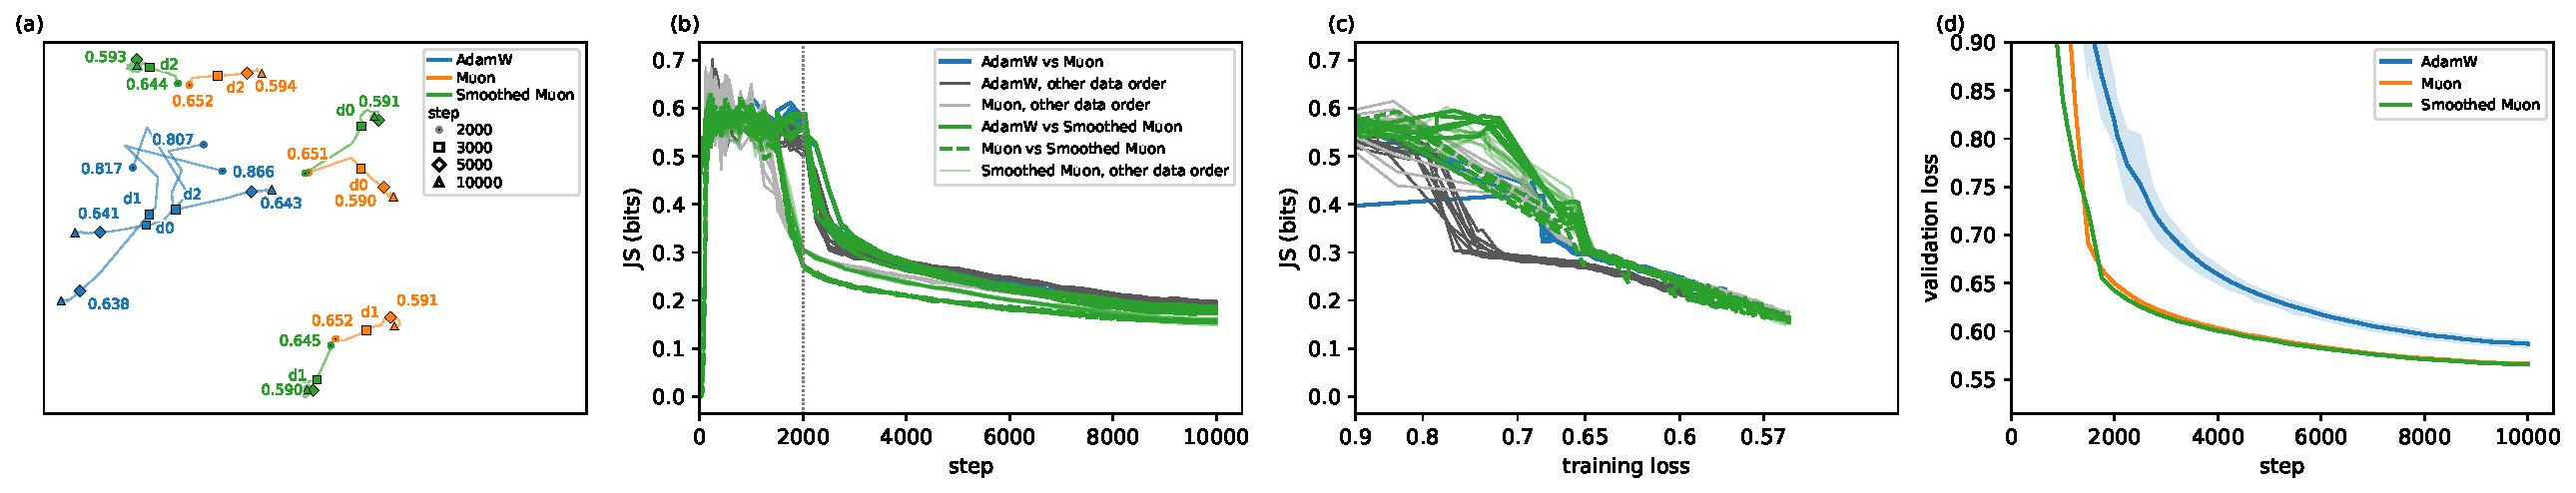
\includegraphics[width=\linewidth]{ts10m_mse_smooth/divergence_umap.pdf}
\caption{AdamW, Muon and smoothed Muon. (a) Next-token predictions of the saved models from step 2000 on, mapped to
2-D by densMAP (shows neighbours, not distances); labels: training loss and data order. (b) JS between runs at equal
step. Blue: AdamW against Muon. Thick green: smoothed Muon against AdamW (solid) and against Muon (dashed), on the same
data order. Grey and thin green: floors (one optimizer, two data orders). Dotted line: step 2000, where (a) starts. (c) The
same at equal training loss. (d) Validation loss; bands: range over data orders.}
\label{fig:div}
\end{figure}

\emph{Speed and endpoints: Muon's.} AdamW's final validation loss (0.587 on average) is reached by smoothed Muon
at step 5500 and by Muon at step 5750 (d). The final validation loss is 0.566 for smoothed Muon, 0.567 for Muon and 0.587 for
AdamW. Over the five data orders it ranges from 0.5646 to 0.5664 for smoothed Muon and from 0.5648 to 0.5679 for Muon,
so the two do not differ.

\emph{Path: Muon's.} Run on the same data order, smoothed Muon and Muon are closer than two Muon runs on different
data orders. At step 5000
their distance is 0.195, and the floors are 0.233 (Muon) and 0.220 (smoothed Muon). At the end it is 0.156: below Muon's
floor (0.175) and equal to smoothed Muon's (0.157); AdamW's floor is 0.192 (b). The same holds at equal loss (c). In (a), each smoothed-Muon run
lies next to the Muon run of its data order. Smoothed Muon is as far from AdamW as Muon is: 0.250 at step 5000 and
0.179 at the end, where Muon is at 0.252 and 0.188.

\paragraph{Step 2: what differs along the way.} We measure the 30 properties of the MSE checkpoint at 34 points of
training, in five groups (\cref{app:metrics} defines them; \cref{tab:app-am,tab:app-sgd} give all values).
\Cref{fig:rank} shows two ratios at training loss 0.65, for the metrics of the MSE checkpoint's figure: AdamW/Muon and
smoothed Muon/Muon, on data orders 0--2 (the ones with these measurements). A green point at 1 means ``as Muon''; a
green point on the black one means ``as AdamW''.

\begin{figure}[H]
\centering
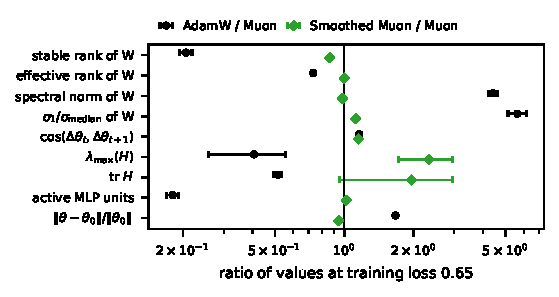
\includegraphics{ts10m_mse_smooth/ranking.pdf}
\caption{Ratios to Muon at training loss 0.65, for selected metrics; three data orders each; bars: range across data
orders. At this loss smoothed Muon's early high curvature is still falling; later its $\operatorname{tr}H$ is below Muon's
(text, \cref{tab:app-curv}).}
\label{fig:rank}
\end{figure}

\begin{itemize}
\item \emph{Weights $W$: Muon's.} The stable rank is 74 (Muon 85, AdamW 17), the effective rank 320 (320, 234), the
spectral norm 2.0 (2.0, 9.1) and $\sigma_1/\sigma_{\rm median}$ 3.2 (2.9, 16.5). The distance from the initialization
is 1.5 times the initial norm (1.6, 2.7).
\item \emph{One-step updates $\Delta\theta$.} The cosine between consecutive steps is AdamW's, as chosen: 0.877 against
0.881 on average over the three data orders (Muon 0.760). It still matches AdamW's at the end: 0.898 against 0.896
(Muon 0.807). The step size and the rank of
$\Delta W$ are Muon's (\cref{tab:app-am}). The step points less along the negative gradient than under either other
optimizer: cosine 0.11, against 0.16 (Muon) and 0.19 (AdamW).
\item \emph{Loss curvature (Hessian $H$; \cref{tab:app-curv}).} Every run starts with a phase of high curvature. Under
smoothed Muon it ends about 500 steps later than under Muon: its top Hessian eigenvalue $\lambda_{\max}$ falls from 1287
to 186 between steps 1500 and 2000, and Muon's from 1239 to 111 between steps 1000 and 1500. Smoothed Muon reaches loss
0.65 just before step 2000, during this fall. So \cref{fig:rank} and \cref{tab:app-am} show its curvature above Muon's
($\lambda_{\max}$ 246 against 107). Later smoothed Muon's $\lambda_{\max}$ is lower on average (154 against 227 at step 4000), but from step 5000 on
the ranges over data orders overlap: at the end, smoothed Muon's is 352 (209 to 461) and Muon's 392 (377 to 402);
AdamW's is 26. The trace does separate. From step 3000 on,
$\operatorname{tr}H$ of smoothed Muon is more than half-way from Muon's to AdamW's (0.53 to 0.84 of the way): at the
end it is 5260 (Muon 8650, AdamW 2210).
\item \emph{Internal activations: Muon's.} 44\% of the MLP units are active, that is, have a positive input (Muon
43\%, AdamW 8\%). The RMS of the residual stream is 1.1 (Muon 1.4, AdamW 40).
\item \emph{Predictions.} At loss 0.65, smoothed Muon's are the least concentrated (entropy 5.30 nats; Muon 4.95,
AdamW 4.59). At loss 0.60 they are next to Muon's (4.17; Muon 4.24, AdamW 3.95).
\end{itemize}

\paragraph{Step 3: swaps (\cref{fig:swap}).} \emph{Swaps.} A \emph{swap} switches a run of one optimizer (the
\emph{parent}, on data order 0) to another optimizer at a \emph{fork step}, then trains it to step 10{,}000 on the
parent's batches (\cref{app:forks}). An optimizer's \emph{own run} is its run from the start. We swap at nine fork steps
from 50 to 4000, in both directions, between every two of the three optimizers: 54 swaps, of which the 18 between
AdamW and Muon are those of the MSE checkpoint. The \emph{fraction} of a swap, for one metric, is its value at step
10{,}000 on a linear scale from the parent's value (0) to that of the new optimizer's own run (1).

\begin{figure}[H]
\centering
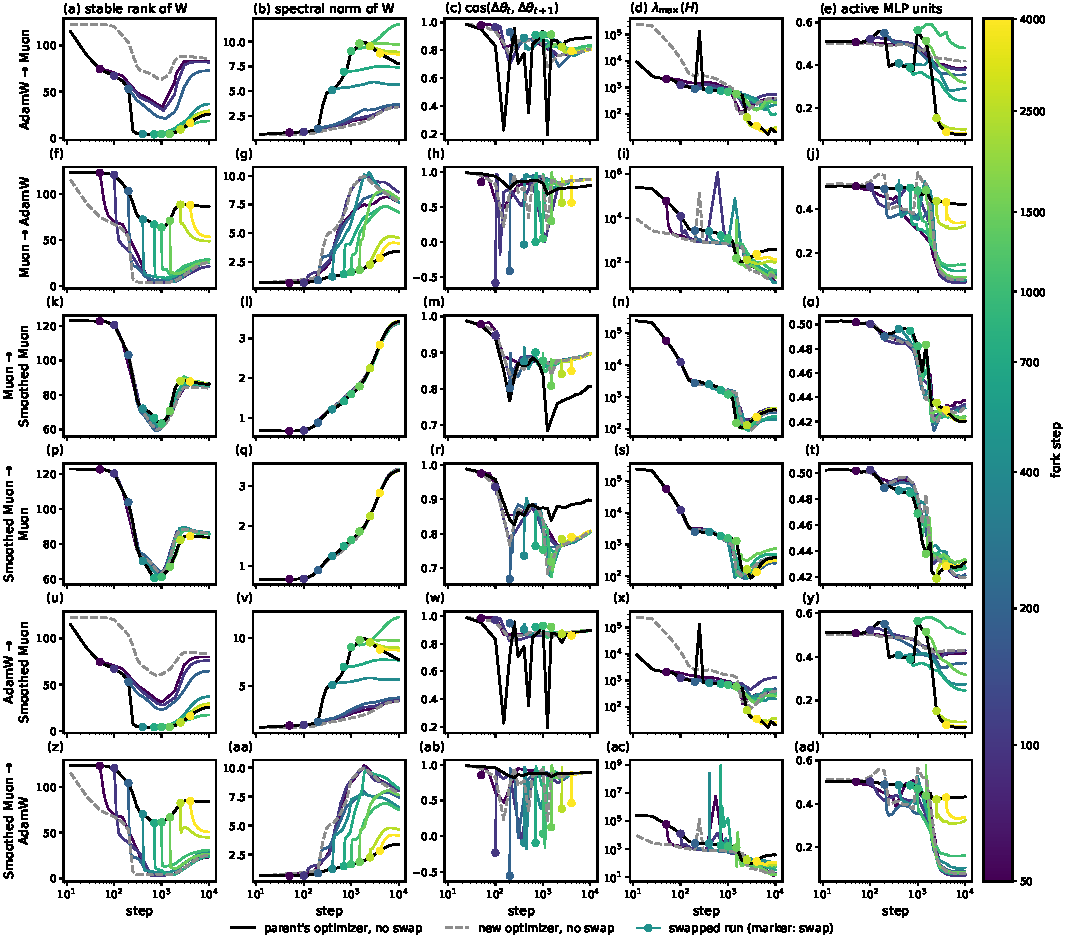
\includegraphics[width=\linewidth]{ts10m_mse_smooth/swap_traj.pdf}
\caption{Swaps on data order 0: five metrics against the step, one row per direction. Black: the parent's optimizer
without a swap; grey dashed: the new optimizer's own run; colour: swapped runs, by fork step (dot: the swap). Before
step 2000, AdamW's $\lambda_{\max}$ spikes and its cosine dips, in its own run and after swaps to it.}
\label{fig:swap}
\end{figure}

\emph{Against AdamW, smoothed Muon swaps as Muon does (u--ad against a--j).} Swaps from AdamW to smoothed Muon at fork
steps 50 to 200, before AdamW's stable rank falls, end most of the way to smoothed Muon's stable rank (fractions 0.93,
0.86 and 0.67; to Muon 0.94, 0.93 and 0.78). Later ones stay near AdamW's (at most 0.20; to Muon 0.19). Swaps from smoothed
Muon to AdamW up to step 1500 end at AdamW's stable rank (0.90 to 1.04), and those at steps 2500 and 4000 about
half-way (0.67 and 0.57; from Muon 0.62 and 0.54). For the stable rank and the share of active MLP units, every
swap's fraction changes by at most 0.12 when Muon replaces smoothed Muon. $\lambda_{\max}$ also
behaves as with Muon: swaps from AdamW at steps 2500 and 4000 stay at AdamW's level (0.05 and 0.01), and swaps to
AdamW end 0.76 to 1.01 of the way.

\emph{Between Muon and smoothed Muon, the cosine and the trace move (k--t).} The own runs of the two agree on the
weights and the MLP, and so do all 18 swaps: stable rank 84 to 87, 42\% to 44\% of MLP units active. The cosine
between consecutive updates ends at the new optimizer's level in all 18: 0.896 to 0.899 after a switch to smoothed
Muon and 0.805 to 0.808 after a switch to Muon (own runs: 0.897 and 0.807). $\lambda_{\max}$ ends between 200 and 740,
in no order of the fork step (own runs: Muon 397, smoothed Muon 385). The Hessian trace, 8940 for Muon and 5040 for smoothed Muon on
this data order, depends on the fork step (\cref{tab:app-swaptrace}): the later the swap, the closer the trace stays
to the parent's. Swaps to smoothed Muon at steps 50, 1500 and 4000 end at 5120, 6990 and 8150 (fractions 0.98, 0.50
and 0.20); swaps to Muon end at 8500, 6840 and 5690 (0.89, 0.46 and 0.17).

\paragraph{Next steps.} (i)~Giving Muon AdamW's cosine did not move its speed, path, weight spectra or MLP sparsity
towards AdamW's, and did not change how it swaps with AdamW. So matching the cosine by averaging does not close these gaps
between Muon and AdamW; the orthogonalization itself is one remaining candidate. (ii)~Find why smoothing lowers the
final Hessian trace by 40\% but $\lambda_{\max}$ by only 10\%, less than its spread over data orders.

\clearpage
\printbibliography

\clearpage
\appendix
%% Appendix of smoothed_muon.tex, \input right after \appendix.
\crefalias{section}{appendix}\crefalias{subsection}{appendix}
\section{Hyperparameters}
\label{app:hparams}

\begin{center}\small
\captionsetup{type=table}
\caption{Hyperparameters shared by the AdamW, Muon and smoothed-Muon runs.}
\label{tab:app-shared}
\begin{tabular}{@{}lp{0.74\linewidth}@{}}
\hline
Runs & AdamW, Muon and smoothed Muon $\times$ data orders d0--d4 (15); the AdamW and Muon runs are those of the MSE
  checkpoint \\
\hline
Model & nanoGPT, pre-LayerNorm blocks \\
Layers, heads, width & 6, 6, 384 \\
MLP & GELU, width 1536 \\
Biases, dropout & none, none \\
Output head & untied \\
Attention projections & separate query, key, value \\
Context & 256 tokens \\
Parameters & 13.9M (10.6M without token and position embeddings and head) \\
\hline
Data & TinyStories (GPT-4 version) \\
Tokenizer & byte-level BPE, 4096 tokens, trained on the training split \\
Batch & 128 windows $\times$ 256 tokens \\
Window offsets & from the training split; generator seeded with (data order, step), same for every optimizer \\
\hline
Loss & MSE: $\|z-e_y\|^2$, summed over the 4096 outputs $z$ (no softmax) and averaged over positions; $e_y$ is the
  one-hot vector of the next token \\
Steps & 10{,}000 \\
Tokens & 328M (about 0.6 epochs) \\
Learning rate & $\eta\,\varphi(t)$ at step $t$, every parameter group \\
Warmup & linear, $\varphi(t)=(t+1)/200$ for $t<200$ \\
Decay & cosine to $\varphi=0.1$ at step 10{,}000 \\
Gradient clipping & none \\
\hline
Initialization seed & 0, all runs \\
Training precision & bfloat16 autocast \\
Prediction, Hessian precision & float32, no autocast (TF32 matrix products allowed) \\
\hline
Logged predictions & next-token distributions $p=\max(z,0)/\sum_v\max(z_v,0)$ (uniform if no output is positive):
  128 fixed validation sequences $\times$ 16 evenly spaced positions (2{,}048), stored as float16 outputs $z$ \\
Training loss & 64 fixed training sequences, all positions; used to match runs at equal loss \\
Floor & mean JS between two data orders of one optimizer, at equal training loss \\
Both logged at & every 250th step $+$ 30 log-spaced steps in $[1, 10{,}000]$ \\
\hline
Hessian & top eigenvalue, 20 Lanczos iterations, 32 fixed training sequences \\
Measured at & every 500th step $+$ 30 log-spaced steps \\
\hline
\end{tabular}
\end{center}

\begin{center}\small
\captionsetup{type=table}
\caption{Optimizer-specific hyperparameters. $n_{\rm out}$, $n_{\rm in}$: output and input size of the matrix.
Smoothed Muon differs from Muon in the rows ``Step'' and $\eta$ only.}
\label{tab:app-optim}
\setlength{\tabcolsep}{4pt}
\begin{tabular}{@{}p{0.15\linewidth}p{0.25\linewidth}p{0.27\linewidth}p{0.27\linewidth}@{}}
\hline
 & AdamW & Muon & Smoothed Muon \tabularnewline
\hline
$\eta$ & $2\cdot10^{-3}$ & $5\cdot10^{-3}$ & $5\cdot10^{-3}$ \tabularnewline
$\eta$ choice & \raggedright second-best final validation loss of a 5-rate sweep on d0 (0.591); the best rate,
  $4\cdot10^{-3}$ (0.584), does not train on d1 (loss stays at 0.86) & \raggedright best final validation loss of a 7-rate sweep on d0 &
  \raggedright best final validation loss of a 5-rate sweep on d0 with $a=0.6$ (\cref{tab:app-lr}) \tabularnewline
Update $O_t$ & bias-corrected moments & \raggedright Nesterov momentum; 5 quintic Newton--Schulz steps in bfloat16 &
  as Muon \tabularnewline
Step & $-\eta\,O_t$ & $-\eta\,O_t$ & \raggedright $-\eta\,U_t/(1-(1-a)^t)$, $U_t=(1-a)U_{t-1}+aO_t$, $a=0.6$
  \tabularnewline
Momentum & $\beta=(0.9,0.95)$ & $\beta=0.95$ & as Muon \tabularnewline
$\epsilon$ & $10^{-8}$ & -- & -- \tabularnewline
Update scale & -- & $\sqrt{\max(1,n_{\rm out}/n_{\rm in})}$ & as Muon \tabularnewline
Weight decay & \raggedright 0.1, decoupled; none on LayerNorm gains & none & none \tabularnewline
Parameters & all & \raggedright query, key, value, attention-output and both MLP matrices of every block & as Muon
  \tabularnewline
\hline
Aux.\ AdamW & -- & embeddings, head, LayerNorm gains & as Muon \tabularnewline
Aux.\ $\eta$, $\beta$, $\epsilon$ & -- & $2\cdot10^{-3}$, $(0.9,0.95)$, $10^{-8}$ & as Muon \tabularnewline
Aux.\ weight decay & -- & none & none \tabularnewline
\hline
\end{tabular}
\end{center}

\section{Calibration of smoothed Muon}
\label{app:calib}

We chose the smoothing constant $a$ and then the learning rate $\eta$ from runs on data order 0, as in
\cref{tab:app-shared} but without Hessian measurements. The cosine between consecutive updates,
$\cos(\Delta\theta_t,\Delta\theta_{t+1})$ with $\Delta\theta_t=\theta_{t+1}-\theta_t$, comes from checkpoints at
$t,t+1,t+2$. \Cref{tab:app-calib,tab:app-lr} give it at training loss 0.65 (interpolated between the checkpoints) and
as its mean over the eight values of $t$ from 3000 to 9998, for all parameters (the metric of Step 2) and for the 36
block matrices alone. These matrices are the only parameters whose update rule differs between Muon and smoothed Muon.
The other parameters are trained by AdamW under all three optimizers, and their cosine is 0.87--0.88 in every run.
With $a=0.6$ the block matrices alone also match AdamW at loss 0.65 (0.889 against 0.884), and their cosine barely
depends on $\eta$ (\cref{tab:app-lr}).

\begin{center}\small
\captionsetup{type=table}
\caption{Choice of $a$: smoothed Muon at Muon's learning rate $\eta=0.005$, data order 0. Bold: the chosen value.}
\label{tab:app-calib}
\begin{tabular}{@{}l|cc|cc|c@{}}
 & \multicolumn{2}{c|}{cosine, all parameters} & \multicolumn{2}{c|}{cosine, block matrices} & final \\
 & at loss 0.65 & steps 3000--9998 & at loss 0.65 & steps 3000--9998 & validation loss \\
\hline
Muon ($a=1$) & 0.759 & 0.790 & 0.666 & 0.694 & 0.5648 \\
$a=0.8$ &0.830 & 0.851 & 0.796 & 0.812 & 0.5654 \\
$a=0.75$ &0.841 & 0.862 & 0.824 & 0.835 & 0.5655 \\
$a=0.7$ &0.854 & 0.872 & 0.847 & 0.858 & 0.5659 \\
$a=0.65$ &0.866 & 0.881 & 0.867 & 0.877 & 0.5652 \\
{\boldmath$a=0.6$} &0.878 & 0.889 & 0.889 & 0.895 & 0.5646 \\
$a=0.5$ &0.869 & 0.902 & 0.917 & 0.926 & 0.5658 \\
$a=0.4$ &0.888 & 0.908 & 0.951 & 0.951 & 0.5676 \\
\hline
AdamW & 0.882 & 0.884 & 0.884 & 0.886 & 0.5908 \\
\hline
\end{tabular}
\end{center}

\begin{center}\small
\captionsetup{type=table}
\caption{Choice of $\eta$: smoothed Muon with $a=0.6$, data order 0. Bold: the chosen value.}
\label{tab:app-lr}
\begin{tabular}{@{}l|cc|cc|c@{}}
 & \multicolumn{2}{c|}{cosine, all parameters} & \multicolumn{2}{c|}{cosine, block matrices} & final \\
$\eta$ & at loss 0.65 & steps 3000--9998 & at loss 0.65 & steps 3000--9998 & validation loss \\
\hline
0.00125 & 0.858 & 0.887 & 0.889 & 0.894 & 0.5740 \\
0.0025 & 0.836 & 0.887 & 0.881 & 0.894 & 0.5669 \\
\textbf{0.005} & 0.878 & 0.889 & 0.889 & 0.895 & 0.5646 \\
0.01 & 0.887 & 0.893 & 0.893 & 0.896 & 0.5664 \\
0.02 & 0.892 & 0.895 & 0.893 & 0.896 & 0.5686 \\
\hline
\end{tabular}
\end{center}

\section{Metrics}
\label{app:metrics}

The Step-2 runs save checkpoints every 1000 steps, at 12 log-spaced steps, and at three consecutive steps $t,t+1,t+2$
for 24 values of $t$ from 25 to 9998 (to measure one-step updates); we measure the metrics at 34 of these per run, and
the Step-3 swaps at the steps in \cref{tab:app-forks}. \emph{Weights}: for all parameters together, $\|\theta\|_2$,
$\|\theta-\theta_0\|/\|\theta_0\|$ and $\|\theta\|_\infty/\|\theta\|_2$; and, averaged over the 36 weight matrices
$W$ of the blocks, the stable rank $\|W\|_F^2/\|W\|_2^2$, the effective rank $\exp H(\sigma/\textstyle\sum\sigma)$
with $H$ the entropy of the normalized singular values $\sigma$, the spectral norm, and $\sigma_1/\sigma_{\rm median}$.
\emph{Updates} $\Delta\theta_t=\theta_{t+1}-\theta_t$: $\|\Delta\theta_t\|/\|\theta_t\|$, its cosine with
$\Delta\theta_{t+1}$ and with the negative gradient $-g_t$ on step $t$'s batch, and the stable and effective rank of
its block matrices $\Delta W$. \emph{Curvature} of the training loss on 32 fixed training sequences, with Hessian $H$:
$\lambda_{\max}(H)$ (20 Lanczos iterations, logged during training), $\operatorname{tr}H$ (10 Rademacher probes),
$\operatorname{tr}H/\lambda_{\max}$, and the batch sharpness $\mathbb{E}_B[g_B^\top H_Bg_B]/\mathbb{E}_B\|g_B\|^2$,
where $g_B$ and $H_B$ are the gradient and Hessian on a mini-batch $B$.
\emph{Predictions}, on the 2{,}048 held-out
positions: entropy, mean top-1 probability, calibration error (15 bins), top-1 accuracy, loss on the targets in the top
and the bottom third of training-set frequency and their difference, and JS to the unigram and to the bigram model
of the training split. \emph{Activations}, on 32 held-out sequences: attention entropy
and attention on the first token (means over layers, heads and positions), fraction of MLP pre-activations above 0,
RMS of the residual stream after the last block, and effective rank of the centred final features.

SGD, the reference in \cref{tab:app-sgd}, uses heavy-ball momentum 0.9 and learning rate 0.02 (the MSE checkpoint
gives its tuning); everything else is as in \cref{tab:app-shared}. SGD learns little: its training loss ends at 0.96
on all three data orders, and predicting every token by its frequency gives 0.986. So \cref{tab:app-sgd} compares
the four optimizers at training loss 0.97, which the other three pass before step 1500.

\begin{center}\small\begin{minipage}{\linewidth}\centering
\captionsetup{type=table}
\caption{All metrics of Step 2 at training loss 0.65, which AdamW reaches near step 4600, Muon near step 2000 and
smoothed Muon (S-Muon) near step 2000: mean $\pm$ half-range over data orders 0--2, and the ratios AdamW/Muon (A/M)
and smoothed Muon/Muon (S/M). If one optimizer's values range over $[a_{\min},a_{\max}]$ and Muon's over
$[b_{\min},b_{\max}]$, the ratio ranges over $[a_{\min}/b_{\max},\,a_{\max}/b_{\min}]$, given as midpoint $\pm$
half-width. Rows marked ($\times10^k$) are in units of $10^k$. Bold: in each ratio column, the five ratios farthest
from 1 whose range excludes 1. At this loss smoothed Muon's early high curvature is still falling (Step 2), which
raises its curvature rows.}
\label{tab:app-am}
\footnotesize\setlength{\tabcolsep}{2.5pt}\setlength{\aboverulesep}{0pt}\setlength{\belowrulesep}{0pt}%
\renewcommand{\arraystretch}{1.15}%
\begin{tabular}{@{}l|ccc|cc@{}}
 & AdamW & Muon & S-Muon & A/M & S/M \\
\midrule
\emph{Weights $W$} & & & & & \\
weight norm $\|\theta\|_2$ & $260 \pm 4$ & $172 \pm 0$ & $163 \pm 1$ & $1.51 \pm 0.03$ & $0.946 \pm 0.007$ \\
distance from init.\ $/\|\theta_0\|$ & $2.68 \pm 0.05$ & $1.61 \pm 0.01$ & $1.52 \pm 0.01$ & $1.67 \pm 0.04$ & $0.945 \pm 0.009$ \\
largest entry $/\|\theta\|_2$ ($\times10^{-3}$) & $7.56 \pm 0.33$ & $8.02 \pm 0.05$ & $7.30 \pm 0.11$ & $0.935 \pm 0.046$ & $0.915 \pm 0.019$ \\
stable rank of $W$ & $17.2 \pm 1.0$ & $85.5 \pm 0.6$ & $73.8 \pm 0.3$ & {\boldmath\textbf{$0.206 \pm 0.013$}} & $0.865 \pm 0.009$ \\
effective rank of $W$ & $234 \pm 4$ & $320 \pm 0$ & $320 \pm 0$ & $0.734 \pm 0.012$ & $0.999 \pm 0.000$ \\
spectral norm of $W$ & $9.11 \pm 0.40$ & $2.04 \pm 0.00$ & $2.00 \pm 0.01$ & $4.42 \pm 0.20$ & $0.982 \pm 0.006$ \\
$\sigma_1/\sigma_{\rm median}$ of $W$ & $16.5 \pm 1.3$ & $2.87 \pm 0.02$ & $3.22 \pm 0.01$ & {\boldmath\textbf{$5.64 \pm 0.51$}} & $1.12 \pm 0.01$ \\
\emph{One-step updates $\Delta W$} & & & & & \\
step size $\|\Delta\theta\|/\|\theta\|$ ($\times10^{-3}$) & $3.51 \pm 0.13$ & $4.81 \pm 0.01$ & $4.78 \pm 0.01$ & $0.727 \pm 0.028$ & $0.994 \pm 0.003$ \\
stable rank of $\Delta W$ & $11.4 \pm 1.0$ & $208 \pm 1$ & $197 \pm 1$ & {\boldmath\textbf{$(5.45 \pm 0.49){\times}10^{-2}$}} & $0.946 \pm 0.007$ \\
effective rank of $\Delta W$ & $195 \pm 5$ & $361 \pm 1$ & $352 \pm 1$ & $0.542 \pm 0.015$ & $0.975 \pm 0.004$ \\
cosine of consecutive steps & $0.881 \pm 0.002$ & $0.760 \pm 0.000$ & $0.877 \pm 0.002$ & $1.16 \pm 0.00$ & $1.15 \pm 0.00$ \\
cosine of step and $-g$ & $0.185 \pm 0.005$ & $0.156 \pm 0.003$ & $0.107 \pm 0.006$ & $1.20 \pm 0.06$ & {\boldmath\textbf{$0.691 \pm 0.054$}} \\
\emph{Loss curvature (Hessian $H$)} & & & & & \\
top Hessian eigenvalue & $40.4 \pm 11.6$ & $107 \pm 10$ & $246 \pm 42$ & $0.407 \pm 0.148$ & {\boldmath\textbf{$2.33 \pm 0.61$}} \\
batch sharpness & $2.20 \pm 0.25$ & $10.1 \pm 3.0$ & $43.8 \pm 16.9$ & $0.272 \pm 0.113$ & {\boldmath\textbf{$6.20 \pm 3.78$}} \\
Hessian trace & $2260 \pm 50$ & $4380 \pm 90$ & $7190 \pm 4200$ & $0.514 \pm 0.021$ & $1.95 \pm 1.00$ \\
trace / top eigenvalue & $58.2 \pm 16.5$ & $41.1 \pm 4.0$ & $19.9 \pm 2.5$ & $1.42 \pm 0.53$ & {\boldmath\textbf{$0.471 \pm 0.103$}} \\
\emph{Internal activations} & & & & & \\
attention entropy (nats) & $2.36 \pm 0.30$ & $3.75 \pm 0.00$ & $3.65 \pm 0.02$ & $0.628 \pm 0.080$ & $0.975 \pm 0.007$ \\
attention on first token ($\times10^{-2}$) & $1.38 \pm 0.07$ & $1.52 \pm 0.01$ & $1.73 \pm 0.04$ & $0.917 \pm 0.052$ & $1.14 \pm 0.03$ \\
active MLP units ($\times10^{-1}$) & $0.792 \pm 0.043$ & $4.34 \pm 0.01$ & $4.45 \pm 0.05$ & {\boldmath\textbf{$0.180 \pm 0.011$}} & $1.02 \pm 0.02$ \\
residual-stream RMS & $40.1 \pm 3.6$ & $1.36 \pm 0.00$ & $1.08 \pm 0.01$ & {\boldmath\textbf{$29.7 \pm 2.7$}} & {\boldmath\textbf{$0.793 \pm 0.012$}} \\
effective rank of features & $231 \pm 2$ & $243 \pm 1$ & $222 \pm 3$ & $0.951 \pm 0.012$ & $0.911 \pm 0.016$ \\
\emph{Predictions} & & & & & \\
prediction entropy (nats) & $4.59 \pm 0.01$ & $4.95 \pm 0.01$ & $5.30 \pm 0.05$ & $0.926 \pm 0.004$ & $1.07 \pm 0.01$ \\
mean top-1 probability & $0.306 \pm 0.002$ & $0.282 \pm 0.001$ & $0.249 \pm 0.005$ & $1.09 \pm 0.01$ & $0.881 \pm 0.022$ \\
calibration error & $0.165 \pm 0.004$ & $0.180 \pm 0.004$ & $0.217 \pm 0.005$ & $0.919 \pm 0.045$ & $1.21 \pm 0.06$ \\
top-1 accuracy & $0.470 \pm 0.004$ & $0.461 \pm 0.003$ & $0.466 \pm 0.002$ & $1.02 \pm 0.02$ & $1.01 \pm 0.01$ \\
loss on frequent targets & $0.378 \pm 0.007$ & $0.379 \pm 0.005$ & $0.379 \pm 0.004$ & $1.00 \pm 0.03$ & $0.999 \pm 0.025$ \\
loss on rare targets & $0.987 \pm 0.004$ & $0.997 \pm 0.002$ & $0.997 \pm 0.001$ & $0.989 \pm 0.006$ & $0.999 \pm 0.003$ \\
rare minus frequent loss & $0.609 \pm 0.011$ & $0.619 \pm 0.007$ & $0.617 \pm 0.005$ & $0.979 \pm 0.028$ & $0.998 \pm 0.018$ \\
JS to unigram model & $0.564 \pm 0.003$ & $0.568 \pm 0.002$ & $0.566 \pm 0.005$ & $0.995 \pm 0.007$ & $0.997 \pm 0.012$ \\
JS to bigram model & $0.466 \pm 0.003$ & $0.487 \pm 0.001$ & $0.518 \pm 0.002$ & $0.954 \pm 0.008$ & $1.06 \pm 0.01$ \\
\end{tabular}\end{minipage}
\end{center}

\begin{center}\small\begin{minipage}{\linewidth}\centering
\captionsetup{type=table}
\caption{The metrics of \cref{tab:app-am} at training loss 0.97, with SGD as a reference: ratios AdamW/SGD (A/S),
Muon/SGD (M/S) and smoothed Muon/SGD (S-M/S). Bold: in each ratio column, the five ratios farthest from 1 whose range
excludes 1.}
\label{tab:app-sgd}
\scriptsize\setlength{\tabcolsep}{2pt}\setlength{\aboverulesep}{0pt}\setlength{\belowrulesep}{0pt}%
\renewcommand{\arraystretch}{1.15}%
\resizebox{\linewidth}{!}{\begin{tabular}{@{}l|cccc|ccc@{}}
 & AdamW & Muon & S-Muon & SGD & A/S & M/S & S-M/S \\
\midrule
\emph{Weights $W$} & & & & & & & \\
weight norm $\|\theta\|_2$ & $155 \pm 10$ & $126 \pm 0$ & $118 \pm 0$ & $99.9 \pm 0.1$ & $1.53 \pm 0.10$ & $1.26 \pm 0.00$ & $1.18 \pm 0.00$ \\
distance from init.\ $/\|\theta_0\|$ & $1.38 \pm 0.13$ & $0.977 \pm 0.001$ & $0.852 \pm 0.004$ & $0.405 \pm 0.002$ & $3.33 \pm 0.34$ & $2.41 \pm 0.01$ & $2.10 \pm 0.02$ \\
largest entry $/\|\theta\|_2$ ($\times10^{-2}$) & $0.837 \pm 0.050$ & $1.08 \pm 0.01$ & $1.03 \pm 0.01$ & $1.02 \pm 0.00$ & $0.834 \pm 0.049$ & $1.06 \pm 0.01$ & $1.01 \pm 0.01$ \\
stable rank of $W$ & $4.01 \pm 0.14$ & $64.1 \pm 0.3$ & $60.4 \pm 0.2$ & $41.5 \pm 0.1$ & {\boldmath\textbf{$(9.61 \pm 0.35){\times}10^{-2}$}} & $1.55 \pm 0.01$ & $1.46 \pm 0.01$ \\
effective rank of $W$ & $208 \pm 13$ & $315 \pm 0$ & $317 \pm 0$ & $283 \pm 0$ & $0.741 \pm 0.048$ & $1.11 \pm 0.00$ & $1.12 \pm 0.00$ \\
spectral norm of $W$ & $9.54 \pm 1.24$ & $1.62 \pm 0.00$ & $1.54 \pm 0.00$ & $3.90 \pm 0.01$ & $2.42 \pm 0.33$ & $0.415 \pm 0.002$ & $0.396 \pm 0.002$ \\
$\sigma_1/\sigma_{\rm median}$ of $W$ & $39.2 \pm 4.7$ & $3.58 \pm 0.01$ & $3.70 \pm 0.01$ & $23.5 \pm 0.1$ & $1.64 \pm 0.21$ & $0.152 \pm 0.001$ & $0.158 \pm 0.001$ \\
\emph{One-step updates $\Delta W$} & & & & & & & \\
step size $\|\Delta\theta\|/\|\theta\|$ ($\times10^{-3}$) & $5.87 \pm 0.13$ & $6.11 \pm 0.07$ & $6.12 \pm 0.01$ & $0.0183 \pm 0.0050$ & {\boldmath\textbf{$322 \pm 90$}} & {\boldmath\textbf{$335 \pm 90$}} & {\boldmath\textbf{$335 \pm 87$}} \\
stable rank of $\Delta W$ & $2.49 \pm 0.30$ & $63.5 \pm 1.0$ & $46.6 \pm 1.5$ & $1.08 \pm 0.03$ & $2.37 \pm 0.33$ & {\boldmath\textbf{$58.3 \pm 2.4$}} & {\boldmath\textbf{$42.9 \pm 2.5$}} \\
effective rank of $\Delta W$ & $56.9 \pm 6.2$ & $227 \pm 2$ & $223 \pm 2$ & $35.5 \pm 1.1$ & $1.66 \pm 0.22$ & $6.44 \pm 0.24$ & $6.37 \pm 0.24$ \\
cosine of consecutive steps & $0.798 \pm 0.093$ & $0.793 \pm 0.010$ & $0.876 \pm 0.001$ & $0.699 \pm 0.168$ & $1.27 \pm 0.45$ & $1.25 \pm 0.32$ & $1.38 \pm 0.34$ \\
cosine of step and $-g$ ($\times10^{-2}$) & $2.36 \pm 0.36$ & $4.99 \pm 0.10$ & $4.51 \pm 0.02$ & $60.0 \pm 22.7$ & {\boldmath\textbf{$(4.73 \pm 2.31){\times}10^{-2}$}} & $(9.42 \pm 3.61){\times}10^{-2}$ & $(8.44 \pm 3.14){\times}10^{-2}$ \\
\emph{Loss curvature (Hessian $H$)} & & & & & & & \\
top Hessian eigenvalue & $635 \pm 11$ & $1200 \pm 10$ & $1760 \pm 20$ & $139 \pm 32$ & $4.69 \pm 1.13$ & $8.81 \pm 2.03$ & $13.0 \pm 3.1$ \\
batch sharpness & $477 \pm 31$ & $869 \pm 9$ & $1060 \pm 20$ & $93.9 \pm 21.9$ & $5.31 \pm 1.55$ & $9.67 \pm 2.33$ & $11.8 \pm 2.9$ \\
Hessian trace & $(1.83 \pm 0.14){\times}10^{6}$ & $(2.45 \pm 0.01){\times}10^{6}$ & $(2.64 \pm 0.02){\times}10^{6}$ & $(1.62 \pm 0.05){\times}10^{4}$ & {\boldmath\textbf{$113 \pm 12$}} & {\boldmath\textbf{$152 \pm 5$}} & {\boldmath\textbf{$164 \pm 6$}} \\
trace / top eigenvalue & $3080 \pm 130$ & $2110 \pm 60$ & $1520 \pm 10$ & $120 \pm 23$ & {\boldmath\textbf{$27.2 \pm 6.5$}} & {\boldmath\textbf{$18.7 \pm 4.2$}} & {\boldmath\textbf{$13.5 \pm 2.8$}} \\
\emph{Internal activations} & & & & & & & \\
attention entropy (nats) & $1.73 \pm 1.09$ & $4.12 \pm 0.01$ & $4.23 \pm 0.00$ & $4.58 \pm 0.00$ & $0.381 \pm 0.238$ & $0.900 \pm 0.001$ & $0.924 \pm 0.001$ \\
attention on first token ($\times10^{-2}$) & $2.29 \pm 1.11$ & $1.85 \pm 0.01$ & $1.95 \pm 0.03$ & $2.02 \pm 0.00$ & $1.30 \pm 0.55$ & $0.913 \pm 0.005$ & $0.965 \pm 0.014$ \\
active MLP units & $0.430 \pm 0.082$ & $0.477 \pm 0.000$ & $0.482 \pm 0.001$ & $0.465 \pm 0.001$ & $0.932 \pm 0.179$ & $1.03 \pm 0.00$ & $1.04 \pm 0.00$ \\
residual-stream RMS & $274 \pm 89$ & $2.14 \pm 0.01$ & $1.64 \pm 0.01$ & $66.0 \pm 1.5$ & $4.03 \pm 1.45$ & {\boldmath\textbf{$(3.26 \pm 0.09){\times}10^{-2}$}} & {\boldmath\textbf{$(2.49 \pm 0.08){\times}10^{-2}$}} \\
effective rank of features & $33.5 \pm 2.4$ & $105 \pm 1$ & $115 \pm 1$ & $41.8 \pm 2.1$ & $0.810 \pm 0.100$ & $2.55 \pm 0.17$ & $2.79 \pm 0.17$ \\
\emph{Predictions} & & & & & & & \\
prediction entropy (nats) & $7.25 \pm 0.02$ & $7.24 \pm 0.00$ & $7.26 \pm 0.01$ & $6.51 \pm 0.02$ & $1.11 \pm 0.01$ & $1.11 \pm 0.00$ & $1.11 \pm 0.00$ \\
mean top-1 probability ($\times10^{-2}$) & $2.69 \pm 0.10$ & $2.81 \pm 0.03$ & $2.68 \pm 0.06$ & $5.68 \pm 0.14$ & $0.476 \pm 0.028$ & $0.494 \pm 0.017$ & $0.472 \pm 0.022$ \\
calibration error ($\times10^{-1}$) & $1.47 \pm 0.07$ & $3.61 \pm 0.03$ & $3.38 \pm 0.02$ & $0.436 \pm 0.020$ & $3.34 \pm 0.30$ & $8.30 \pm 0.43$ & $7.77 \pm 0.39$ \\
top-1 accuracy & $0.174 \pm 0.007$ & $0.389 \pm 0.003$ & $0.365 \pm 0.002$ & $0.100 \pm 0.001$ & $1.71 \pm 0.08$ & $3.88 \pm 0.05$ & $3.64 \pm 0.04$ \\
loss on frequent targets & $0.780 \pm 0.016$ & $0.662 \pm 0.005$ & $0.669 \pm 0.007$ & $0.879 \pm 0.003$ & $0.887 \pm 0.020$ & $0.751 \pm 0.008$ & $0.760 \pm 0.011$ \\
loss on rare targets & $1.09 \pm 0.01$ & $1.28 \pm 0.00$ & $1.26 \pm 0.00$ & $1.02 \pm 0.00$ & $1.07 \pm 0.01$ & $1.26 \pm 0.00$ & $1.24 \pm 0.00$ \\
rare minus frequent loss & $0.312 \pm 0.022$ & $0.619 \pm 0.006$ & $0.587 \pm 0.008$ & $0.137 \pm 0.004$ & $2.26 \pm 0.22$ & $4.53 \pm 0.17$ & $4.31 \pm 0.18$ \\
JS to unigram model & $0.578 \pm 0.002$ & $0.657 \pm 0.010$ & $0.640 \pm 0.009$ & $0.218 \pm 0.004$ & $2.64 \pm 0.05$ & $3.02 \pm 0.10$ & $2.94 \pm 0.09$ \\
JS to bigram model & $0.758 \pm 0.006$ & $0.793 \pm 0.002$ & $0.789 \pm 0.004$ & $0.648 \pm 0.003$ & $1.17 \pm 0.01$ & $1.23 \pm 0.01$ & $1.22 \pm 0.01$ \\
\end{tabular}}\end{minipage}
\end{center}

\begin{center}\small
\captionsetup{type=table}
\caption{Curvature over training: top Hessian eigenvalue $\lambda_{\max}$ and Hessian trace $\operatorname{tr}H$ at fixed
steps, mean $\pm$ half-range over data orders 0--2.}
\label{tab:app-curv}
\footnotesize\setlength{\tabcolsep}{4pt}
\begin{tabular}{@{}r|ccc|ccc@{}}
 & \multicolumn{3}{c|}{$\lambda_{\max}$} & \multicolumn{3}{c}{$\operatorname{tr}H$} \\
step & AdamW & Muon & S-Muon & AdamW & Muon & S-Muon \\
\hline
500 & $764 \pm 22$ & $2250 \pm 58$ & $2213 \pm 94$ & $(2.61 \pm 0.05){\times}10^6$ & $(2.96 \pm 0.01){\times}10^6$ & $(2.91 \pm 0.01){\times}10^6$ \\
1000 & $919 \pm 376$ & $1239 \pm 38$ & $1617 \pm 17$ & $(2.17 \pm 0.06){\times}10^6$ & $(2.60 \pm 0.01){\times}10^6$ & $(2.45 \pm 0.01){\times}10^6$ \\
1500 & $575 \pm 11$ & $111 \pm 38$ & $1287 \pm 16$ & $(1.76 \pm 0.08){\times}10^6$ & $11994 \pm 410$ & $(1.98 \pm 0.04){\times}10^6$ \\
2000 & $474 \pm 24$ & $107 \pm 8$ & $186 \pm 33$ & $(1.40 \pm 0.20){\times}10^6$ & $4470 \pm 121$ & $3655 \pm 155$ \\
2500 & $733 \pm 967$ & $116 \pm 15$ & $162 \pm 62$ & $2056 \pm 657$ & $3635 \pm 109$ & $2915 \pm 114$ \\
3000 & $126 \pm 91$ & $153 \pm 24$ & $104 \pm 21$ & $2191 \pm 132$ & $3552 \pm 75$ & $2604 \pm 49$ \\
4000 & $52.6 \pm 17.5$ & $227 \pm 11$ & $154 \pm 36$ & $2306 \pm 37$ & $4282 \pm 102$ & $2620 \pm 174$ \\
5000 & $36.4 \pm 7.8$ & $296 \pm 20$ & $223 \pm 70$ & $2250 \pm 35$ & $5096 \pm 46$ & $3052 \pm 156$ \\
6000 & $26.7 \pm 5.4$ & $334 \pm 15$ & $271 \pm 101$ & $2172 \pm 40$ & $5853 \pm 154$ & $3422 \pm 209$ \\
7000 & $18.8 \pm 2.6$ & $373 \pm 15$ & $311 \pm 121$ & $2119 \pm 37$ & $6663 \pm 219$ & $3876 \pm 173$ \\
8000 & $20.4 \pm 5.9$ & $380 \pm 6$ & $327 \pm 126$ & $2151 \pm 36$ & $7273 \pm 262$ & $4367 \pm 239$ \\
9000 & $24.3 \pm 0.3$ & $393 \pm 9$ & $344 \pm 126$ & $2171 \pm 35$ & $8054 \pm 119$ & $4824 \pm 229$ \\
10000 & $26.2 \pm 6.8$ & $392 \pm 13$ & $352 \pm 126$ & $2213 \pm 57$ & $8649 \pm 255$ & $5260 \pm 196$ \\
\hline
\end{tabular}
\end{center}

\section{Swaps}
\label{app:forks}

\begin{center}\small\begin{minipage}{\linewidth}\centering
\captionsetup{type=table}
\caption{Swaps. $A$: parent's optimizer; $B$: optimizer after the swap; $s$: fork step.}
\label{tab:app-forks}
\begin{tabular}{@{}lp{0.74\linewidth}@{}}
\hline
Parents & the d0 runs of AdamW, Muon and smoothed Muon (\cref{tab:app-shared}) \\
Warm state & the other optimizer, stepped on the same mini-batch gradients with learning rate 0: momenta, second
  moments and step counts evolve as if training; parameters follow $A$ alone. The AdamW and Muon parents keep each
  other's state, the smoothed-Muon parent keeps both \\
Fork steps $s$ & 50, 100, 200, 400, 700, 1000, 1500, 2500, 4000 \\
Saved at $s$ & parameters; states of the parent's optimizer and of its warm optimizers \\
\hline
Swap $A\to B$ loads & parameters at $s$; $B$'s warm state \\
Swap to smoothed Muon & the AdamW and Muon parents kept no smoothed-Muon state, so the swap loads Muon's state (momentum
  $M$ and auxiliary AdamW) and restarts the average $U$ at the swap: its first step is Muon's step. $U$ forgets its
  start within a few steps (the weight of a step $k$ steps back is $a(1-a)^k$) \\
Hyperparameters & $B$'s (\cref{tab:app-optim}) \\
Steps & $s$ to 10{,}000, on the parent's schedule and batches (data order 0) \\
Swap forks & 6 directions $\times$ 9 steps $=$ 54 (18 between AdamW and Muon, from the MSE checkpoint) \\
Metrics (\cref{fig:swap}) & at $s+{}$0, 5, 10, 25, 50, 100, 250, 500, 1000, 2000, 4000, 6000 (each with the next
  two steps, for the updates) and every 1000 steps \\
\hline
Same-batch control & the parent itself ($A$ continued with the same batches) \\
\hline
\end{tabular}\end{minipage}
\end{center}

\begin{center}\small
\captionsetup{type=table}
\caption{Hessian trace at step 10{,}000 of every swapped run (data order 0). ``Parent'' and ``new'': the own runs of
the parent's and of the new optimizer. The two swaps from AdamW at fork step 1000 end outside the interval between the
own runs, also in other metrics (\cref{fig:swap}); we have not looked into why.}
\label{tab:app-swaptrace}
\footnotesize\setlength{\tabcolsep}{4pt}
\begin{tabular}{@{}l|c|ccccccccc|c@{}}
 & & \multicolumn{9}{c|}{fork step} & \\
swap & parent & 50 & 100 & 200 & 400 & 700 & 1000 & 1500 & 2500 & 4000 & new \\
\hline
AdamW $\to$ Muon & 2257 & 9190 & 8429 & 5726 & 3157 & 1753 & 15463 & 1882 & 2406 & 2179 & 8941 \\
Muon $\to$ AdamW & 8941 & 2178 & 2259 & 2217 & 2398 & 2342 & 2027 & 3167 & 3309 & 3380 & 2257 \\
Muon $\to$ S-Muon & 8941 & 5118 & 5817 & 5175 & 5334 & 6392 & 6269 & 6988 & 7456 & 8152 & 5037 \\
S-Muon $\to$ Muon & 5037 & 8495 & 8508 & 8098 & 7181 & 7433 & 7528 & 6836 & 6039 & 5686 & 8941 \\
AdamW $\to$ S-Muon & 2257 & 5079 & 4925 & 3417 & 2272 & 1935 & 16259 & 1827 & 2362 & 2135 & 5037 \\
S-Muon $\to$ AdamW & 5037 & 2097 & 2269 & 2287 & 2351 & 2600 & 2441 & 2561 & 3047 & 2675 & 2257 \\
\hline
\end{tabular}
\end{center}


\end{document}
